%SSS - move to related work 

Assuming fixed, known recovery times may be adequate for crude time scales (measured in days). The urgency of preventing failure propagation necessitates a finer time scale (minutes or hours) for recovery actions. Deterministic recovery time is an unrealistic assumption on these finer time scales. Exponential assumptions are somewhat more suitable for the timescales, but having an exponential distribution alone is insufficient. The repair time for each component could be in different repair distributions, such as Lognormal ~\cite{l_c_cadwallader_review_2012} and Weibull ~\cite{ocansey_temperature-driven_2025} distributions, even under the same system. So we must consider multiple distributions of repair time in one model.

%SSS - this was in the intro, where we discuss the use of the work in improving network design
, as well as recommending tweaking or enhancements in interdependency to reduce recovery needs in the event of cascading failures. 

The first two can be found in the service provider's database like outage reports or maintenance histories. For example, Ameren's outage map: \url{https://outagemap.ameren.com}, %pretty sure they keep very minute of their activities on file for past months, or even years.
%And outage happens very day, there wil be plenty of data for us to do dependency measure and repair time measure
And the third one can be designed from scratch, or optimized from existing repair schemes. 

\paragraph{Component-level information about failure} is the essential source for identifying the frequent faults that happened in the given system or similar systems. As we study the failure cases in the system, we could statistically analyze the dependencies between components, the consequential faults, and the tight couplings; using methods like correlations~\cite{}, mutual information~\cite{}, and Granger causality~\cite{}. For a specific type of system, there could be some specialized methods to quantify the dependencies, such as Hydraulic measures  for water systems~\cite{}, Spatial-temporal correlation for traffic systems~\cite{}, and aging of components for power systems~\cite{}. 

\paragraph{repair} is the essential source for estimating the repair process. The repair time can usually be found in outage reports~\cite{}. Where the maintenance company provides a timeline of when a component is first attempted to be repaired, and when it was finished. Most service providers will keep their maintenance records to track the time, resources, and labor spent repairing components as part of their economic assessment. The distribution of repair time for each component can be found by statistically analyzing all the reports that contain the repair spent on each component and matching the data points with distribution functions. The 3 commonly used repair time distributions are: Exponential, Lognormal, Weibull distribution as shown in figure\ref{fig:3_distributions}. 
The exponential distribution assumes that the time it takes to repair the failure does not depend on time spent. It is commonly used for small, short-time fixes, such as resetting a breaker, restarting a machine, and rebooting a controlling device. The minimum repair time of exponential distribution is 0 and majority of the distribution are leaning towards 0. A common example would be rebooting controlling/monitoring devices from distance (with wireless command). 

The lognormal distribution assumes the repair is affected by numerous minor multiplicative factors such as delays, logistics, and environmental conditions, resulting in skewed distributions. A common example would be repairing a downed distribution line during a snowstorm. 

The Weibull distribution is similar to lognormal in that it is skewed initially. The repair time is very uncertain as the damage could be minor or severe. Usually for highly reliable systems damaged by extreme weather. A common example would be repairing a high-voltage transmission line after a hurricane. 

\begin{figure}
    \centering
    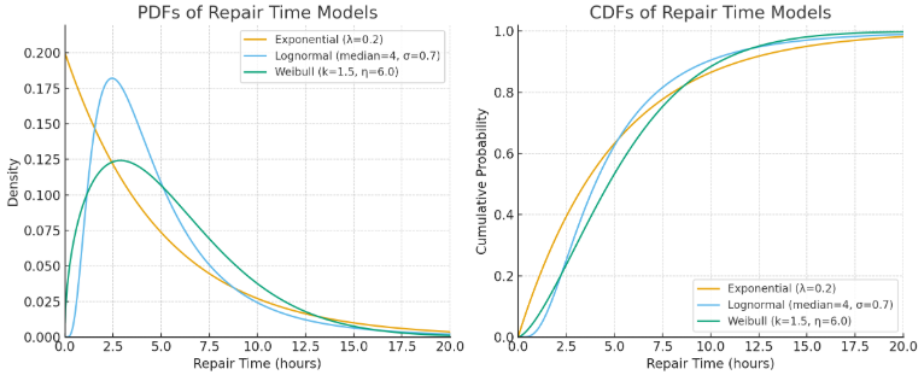
\includegraphics[width=1\linewidth]{images/3_distribtions.png}
    \caption{Exponential, Lognormal, Weibull distribution example}
    \label{fig:3_distributions}
\end{figure}

\paragraph{network topology} is the fundamental structure of the components in the given system as it depicts the connections between components, and how the service should flow between components. It's another source of information to measure dependencies and find the nominal service of the system for performance evaluation. Likely, the topology of the network could also be used to quantify the dependencies between components as well. 
For example, the IEEE test system~\cite{} provides connections between power lines and buses, their normal voltage during operation, and vector of service distribution. 

\paragraph{repair schemes to be tested} is the specific repair plan to be executed during failure of the given system. There are static schemes, and there are dynamical schemes. The static ones are determined in advance that ranks the priority of the components, and the crews will repair them from highest priority to the lowest~\cite{}. The dynamic ones usually require the observation or assessment of the system status and then make a decision based during run time ~\cite{}.